\begin{figure}[t]
\centering
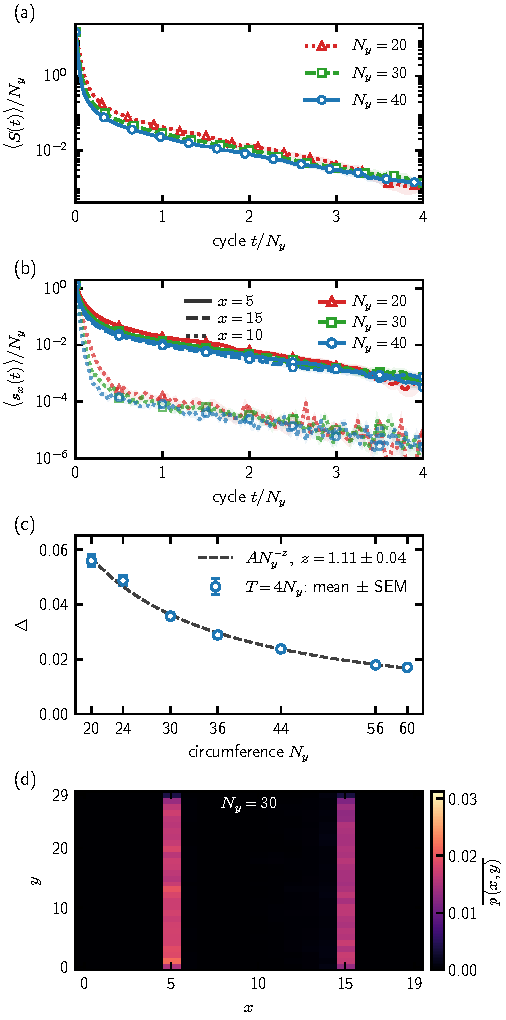
\includegraphics[width=\columnwidth]{hard_wall_purification_contours_gap_density_4x1.pdf}
\caption{Hard-wall purification from a maximally mixed active slab,
$N_x=20$, $\alpha_1=1$, $\alpha_2=30$, $n_{\rm shell}=1$,
with perfect correction and 100 independent Born trajectories per size.
(a) Mean total entropy per $N_y$.
(b) Mean entropy contours summed over $y$ and orbitals, at the walls
($x=5,15$) and center ($x=10$). Bands denote one sample SEM.
(c) Mean endpoint gap $\Delta=\min_j|\operatorname{atanh}(a_j)|/(4N_y)$,
with centered covariance eigenvalues $a_j$ and SEM bars.
The fit over all shown sizes gives $\Delta\propto N_y^{-1.11\pm0.04}$.
(d) Endpoint mode probability density at $N_y=30$, $T=4N_y$:
orbital-summed probabilities are averaged over modes with
$10^{-9}<\nu_j<1-10^{-9}$ within each trajectory, then equally over
trajectories. The density sums to one; colors are linear.
All runs end at $T=4N_y$.}
\label{fig:hard-wall-purification-modes}
\end{figure}
